%% =========================================
%%      PLANTILLA INFORMES AST-FIZ UC
%% =========================================
%% 
%% [UC-TeX] You will find two kind of tags before each comment. %% [UC-TeX] or %% [AASTeX], 
%% [UC-TeX] %% [UC-TeX] means that was updated by us and %% [AASTeX] means that was taken from AASTeX.
%% [UC-TeX] You will also find comments with the tag %% [INPUT] which means that you have to input something there.
%% 
%% [UC-TeX] Modified from AASTeX v7
%% [AASTeX] Version 7. Created January 2025.  
%% 
%% [AASTeX] AASTeX v7 calls the following external packages:
%% [AASTeX] times, hyperref, ifthen, hyphens, longtable, xcolor, 
%% [AASTeX] bookmarks, array, rotating, ulem, and lineno 
%% 
%% [AASTeX] RevTeX is no longer used in AASTeX v7.
%% [UC-TeX]: [MOD]s in .cls have been made. Look for them with the [MOD] tag.

%% [UC-TeX][INPUT] 
%% [UC-TeX] You can select from two column or one column mode. Recommended mode is preprint, preprint2 & modern.
\documentclass[preprint]{aastex7}
%% [AASTeX] This initial command takes arguments that can be used to easily modify 
%% [AASTeX] the output of the compiled manuscript. Any combination of arguments can be 
%% [AASTeX] invoked like this:
%% [AASTeX]
%% [AASTeX] \documentclass[argument1,argument2,argument3,...]{aastex7}
%% [AASTeX]
%% [AASTeX] Six of the arguments are typestting options. They are:
%% [AASTeX] 
%% [AASTeX]  twocolumn   : two text columns, 10 point font, single spaced article.
%% [AASTeX]                This is the most compact and represent the final published
%% [AASTeX]                derived PDF copy of the accepted manuscript from the publisher
%% [AASTeX]  default     : one text column, 10 point font, single spaced (default).
%% [AASTeX]  manuscript  : one text column, 12 point font, double spaced article.
%% [AASTeX]  preprint    : one text column, 12 point font, single spaced article.  
%% [AASTeX]  preprint2   : two text columns, 12 point font, single spaced article.
%% [AASTeX]  modern      : a stylish, single text column, 12 point font, article with
%% [AASTeX] 		  wider left and right margins. This uses the Daniel
%% [AASTeX] 		  Foreman-Mackey and David Hogg design.
%% [AASTeX] 
%% [AASTeX] Note that you can submit to the AAS Journals in any of these 6 styles.
%% [AASTeX] 
%% [AASTeX] There are other optional arguments one can invoke to allow other stylistic
%% [AASTeX] actions. The available options are:
%% [AASTeX] 
%% [AASTeX]   astrosymb    : Loads Astrosymb font and define \astrocommands. 
%% [AASTeX]   tighten      : Makes baselineskip slightly smaller, only works with 
%% [AASTeX]                  the twocolumn substyle.
%% [AASTeX]   times        : uses times font instead of the default.
%% [AASTeX]   linenumbers  : turn on linenumbering. Note this is mandatory for AAS
%% [AASTeX]                  Journal submissions and revisions.
%% [AASTeX]   trackchanges : Shows added text in bold.
%% [AASTeX]   longauthor   : Do not use the more compressed footnote style (default) for 
%% [AASTeX]                  the author/collaboration/affiliations. Instead print all
%% [AASTeX]                  affiliation information after each name. Creates a much 
%% [AASTeX]                  longer author list but may be desirable for short 
%% [AASTeX]                  author papers.
%% [AASTeX] twocolappendix : make 2 column appendix.
%% [AASTeX]   anonymous    : Do not show the authors, affiliations, acknowledgments,
%% [AASTeX]                  and author contributions for dual anonymous review.
%% [AASTeX]  resetfootnote : Reset footnotes to 1 in the body of the manuscript.
%% [AASTeX]                  Useful when there are a lot of authors and affiliations
%% [AASTeX] 		    in the front matter.
%% [AASTeX]   longbib      : Print article titles in the references. This option
%% [AASTeX] 		    is mandatory for PSJ manuscripts.
%% [AASTeX] 
%% [AASTeX] Since v6, AASTeX has included \hyperref support. While we have built in 
%% [AASTeX] specific %% defaults into the classfile you can manually override them 
%% [AASTeX] with the \hypersetup command. For example,
%% [AASTeX] 
%% [AASTeX] \hypersetup{linkcolor=red,citecolor=green,filecolor=cyan,urlcolor=magenta}
%% [AASTeX] 
%% [AASTeX] will change the color of the internal links to red, the links to the
%% [AASTeX] bibliography to green, the file links to cyan, and the external links to
%% [AASTeX] magenta. Additional information on \hyperref options can be found here:
%% [AASTeX] https://www.tug.org/applications/hyperref/manual.html#x1-40003
%% [AASTeX] 
%% [AASTeX] The "bookmarks" has been changed to "true" in hyperref
%% [AASTeX] to improve the accessibility of the compiled pdf file.
%% [AASTeX] 
%% [AASTeX] If you want to create your own macros, you can do so
%% [AASTeX] using \newcommand. Your macros should appear before
%% [AASTeX] the \begin{document} command.
%% [AASTeX]
\newcommand{\vdag}{(v)^\dagger}
\newcommand\aastex{AAS\TeX}
\newcommand\latex{La\TeX}

\makeatletter
\let\frontmatter@title@above=\relax
\makeatother
%% [AASTeX] %%%%%%%%%%%%%%%%%%%%%%%%%%%%%%%%%%%%%%%%%%%%%%%%%%%%%%%%%%%%%%%%%%%%%%%%%%%%%% 
%% [AASTeX] 
%% [AASTeX] The following section outlines numerous optional output that
%% [AASTeX] can be displayed in the front matter or as running meta-data.
%% [AASTeX] 
%% [AASTeX] Running header information. A short title on odd pages and 
%% [AASTeX] short author list on even pages. Note that this
%% [AASTeX] information may be modified in production.

%% [UC-TeX] ================================================ COVER =======================================================

%% [UC-TeX] Cover Names
\def\studenttextsingular{Estudiante}
\def\studenttextplural{Estudiantes}
\def\professortextsingular{Profesor}
\def\professortextplural{Profesores}

%% [UC-TeX] Cover Logo (Para modificar el logo puedes usar los predefinidos o importar uno nuevo)
%% [UC-TeX] Logos located at Resources/logos/...
%% [UC-TeX] Coloca la extensión del logo:
%% [UC-TeX][INPUT]
\def\coversubjectlogo{AST-center-black.png} 
\def\coversubjectlogoscale{0.25} 
\def\largetitlename{Laboratorio: Observación de Objetos de Espacio Profundo}

%% [UC-TeX][INPUT] 
%% [UC-TeX] Cover Authors (Ingresa los autores en el formato {ORCID}{Nombre}, ...)
\def\coverauthors{
    {0009-0005-4685-695X}{Norman Pogson},
    {0000-0000-0000-0000}{Richard Fisher}
}

%% [UC-TeX][INPUT] 
%% [UC-TeX] Cover Professors (Ingresa los profesores en el formato {ORCID}{Nombre}, ...)
%% [UC-TeX] Si no hay profesores, tienes que editarlo en Pages/Doc/cover.tex y comentar el \printprof
\def\coverprofessor{
    {0000-0000-0000-0000}{Prof. Henrietta Leavitt}
    % you may add more here (remember the comma)
}

%% [UC-TeX] ================================================ HEADER ======================================================
%% [UC-TeX][INPUT] 
%% [UC-TeX] Text for headers for odd and even pages.
\shorttitle{Laboratorio DSOs}
\shortauthors{Norman Pogson}

%% [AASTeX] Include dates for submitted, revised, and accepted.
%% [AASTeX] \received{February 1, 2025}
%% [AASTeX] \revised{March 1, 2025}
%% [AASTeX] \accepted{\today}
%% [AASTeX] 
%% [AASTeX] Indicate AAS Journal the manuscript was submitted to.
%% [AASTeX] \submitjournal{PSJ}
%% [AASTeX] Note that this command adds "Submitted to " the argument.
%% [AASTeX] 
%% [AASTeX] You can add a light gray and diagonal water-mark to the first page 
%% [AASTeX] with this command:
%% [AASTeX] \watermark{text}
%% [AASTeX] where "text", e.g. DRAFT, is the text to appear.  If the text is 
%% [AASTeX] long you can control the water-mark size with:
%% [AASTeX] \setwatermarkfontsize{dimension}
%% [AASTeX] where dimension is any recognized LaTeX dimension, e.g. pt, in, etc.
%% [AASTeX] %%%%%%%%%%%%%%%%%%%%%%%%%%%%%%%%%%%%%%%%%%%%%%%%%%%%%%%%%%%%%%%%%%%%%%%%%%%%%%%% 
%% [AASTeX] 
%% [AASTeX] Use this command to indicate a subdirectory where figures are located.
%% [AASTeX] \graphicspath{{./}{figures/}}
%% [AASTeX] This is the end of the preamble.  Indicate the beginning of the
%% [AASTeX] manuscript itself with \begin{document}.

%% [UC-TeX] ================================================ IDIOMAS ======================================================
\def\partname{Parte}
\def\tocname{Contenidos}
\def\lofname{Lista de Figuras}
\def\lotname{Lista de Tablas}
\def\refname{Referencias}
\def\indexname{Índice}
\def\figurename{Figura}
\def\figuresname{Figuras}%
\def\tablename{Tabla}
\def\tablesname{Tablas}%
\def\abstractname{Resúmen}
\def\appendixesname{Apéndices}%
\def\appendixname{Apéndice}%
\def\facilitiesname{Lugares}


\begin{document}
%% [UC-TeX][INPUT] 
%% [UC-TeX] Be cautious with the cover page.
\thispagestyle{empty}
\makeatletter
\newcount\authorcount
\def\countauthors{%
    \authorcount=0%
    \@for\@temp:=\coverauthors\do{\advance\authorcount by 1}%
}

% Main
\newcommand{\printauthors}{%
    \countauthors%
    \begin{center}
    \large\textbf{%
        \ifnum\authorcount>1%
            \studenttextplural%
        \else%
            \studenttextsingular%
        \fi%
    }
    \end{center} \vspace{-0.35cm}
    \expandafter\@processauthors\coverauthors,\@nil%
}

% Process author list
\def\@processauthors#1,#2\@nil{%
    \ifx&#1&%
    \else%
        \expandafter\@processauthor#1\\%
        \ifx&#2&%
        \else%
            \@processauthors#2\@nil%
        \fi%
    \fi%
}

\def\@processauthor#1#2\\{%
    \href{https://orcid.org/#1}{\textsc{#2} 
\includegraphics[height=0.8em]{Resources/misc/orcid-ID.png}}\\
}
\makeatother

\makeatletter
\newcount\authorcount
\def\countauthors{%
    \authorcount=0%
    \@for\@temp:=\coverprofessor\do{\advance\authorcount by 1}%
}

% Main
\newcommand{\printprof}{%
    \countauthors%
    \begin{center}
    \large\textbf{%
        \ifnum\authorcount>1%
            \professortextplural%
        \else%
            \professortextsingular%
        \fi%
    }
    \end{center} \vspace{-0.35cm}
    \expandafter\@processauthors\coverprofessor,\@nil%
}

% Process author list
\def\@processauthors#1,#2\@nil{%
    \ifx&#1&%
    \else%
        \expandafter\@processauthor#1\\%
        \ifx&#2&%
        \else%
            \@processauthors#2\@nil%
        \fi%
    \fi%
}

\def\@processauthor#1#2\\{%
    \href{https://orcid.org/#1}{\textsc{#2} 
\includegraphics[height=0.8em]{Resources/misc/orcid-ID.png}}\\
}
\makeatother



\begin{titlepage}
    \newcommand{\HRule}{\rule{\linewidth}{0.5mm}}
    \center
    % \textsc{\LARGE Pontificia Universidad Católica de Chile}\\[1cm] 
    
    \vspace{1.5cm}
    % If you want to override the logo, uncomment the line below and use and comment \coverlogo
    % 
\includegraphics[height=6cm]{Resources/logos/AST-center-black.png}
    \includegraphics[scale=\coversubjectlogoscale]{Resources/logos/\coversubjectlogo}
    
    \vspace{1cm}
    \HRule \\[0.4cm]
    {\huge \bfseries \largetitlename}\\
    \HRule \\
    
    \vfill
    
    \large \textbf{Asignatura} \\
    \textsc{AST101} - Objetos Messier
    
    \vspace{1cm}
    
    % \large \textbf{Estudiante} \\
    \printauthors
    
    \vspace{1cm}
    
    \printprof
    
    \vfill
    
    \begin{minipage}[t]{0.45\textwidth}
        \centering
        \large \textbf{Fecha de la visita} \\ 24 de Abril, \the\year
    \end{minipage}
        \hfill
    \begin{minipage}[t]{0.45\textwidth}
        \centering
        \large \textbf{Fecha de entrega} \\ \the\day \ de Abril, \the\year
    \end{minipage}
    
\end{titlepage}
\newpage

%% [UC-TeX][INPUT] 
%% [UC-TeX] Content Title
\title{\Large{\largetitlename}}

%% [UC-TeX] ================================================ AUTHORS =====================================================
%% [AASTex] A significant change from AASTeX v6+ is in the author blocks. Now an email
%% [AASTex] address is required for each author. This means that each author requires
%% [AASTex] at least one of the following:
%% [AASTex] 
%% [AASTex] \author
%% [AASTex] \affiliation
%% [AASTex] \email
%% [AASTex] 
%% [AASTex] If these three commands are not available for each author, the latex
%% [AASTex] compiler will issue an error and if you force the latex compiler to continue,
%% [AASTex] it will generate an incomplete pdf.
%% [AASTex] 
%% [AASTex] Multiple \affiliation commands are allowed and authors can also include
%% [AASTex] an optional \altaffiliation to indicate a status, i.e. Hubble Fellow. 
%% [AASTex] while affiliations are indexed as footnotes, altaffiliations are noted with
%% [AASTex] with a non-numeric footnote that is set away from the numeric \affiliation 
%% [AASTex] footnotes. NOTE that if an \altaffiliation command is used it must 
%% [AASTex] come BEFORE the \affiliation call, right after the \author command, in 
%% [AASTex] order to place the footnotes in the proper location. Because non-numeric
%% [AASTex] symbols are used, \altaffiliation should be used sparingly.
%% [AASTex] 
%% [AASTex] In v7 the \author command takes an optional argument which provides 
%% [AASTex] additional metadata about the author. Authors can provide the 16 digit 
%% [AASTex] ORCID, the surname (family or last) name, the given (first or fore-) name, 
%% [AASTex] and a name suffix, e.g. "Jr.". The syntax is:
%% [AASTex] 
%% [AASTex] \author[orcid=0000-0002-9072-1121,gname=Gregory,sname=Schwarz]{Greg Schwarz}
%% [AASTex] 
%% [AASTex] This name metadata in not shown, it is only for parsing by the peer review
%% [AASTex] system so authors can be more easily identified. This name information will
%% [AASTex] also be sent to the publisher so they can include it in the CROSSREF 
%% [AASTex] metadata. Including an orcid will hyperlink the author name to the 
%% [AASTex] author's ORCID page. Note that  during compilation, LaTeX will do some 
%% [AASTex] limited checking of the format of the ID to make sure it is valid. If 
%% [AASTex] the "orcid-ID.png" image file is  present or in the LaTeX pathway, the 
%% [AASTex] ORCID icon will appear next to the authors name.
%% [AASTex] 
%% [AASTex] Even though emails are now required for each author, the \email does not
%% [AASTex] produce output in the compiled manuscript unless the optional "show" command
%% [AASTex] is used. For example,
%% [AASTex] 
%% [AASTex] \email[show]{greg.schwarz@aas.org}
%% [AASTex] 
%% [AASTex] All "shown" emails are show in the bottom left of the first page. Due to
%% [AASTex] space constraints, only a few emails should be shown. 
%% [AASTex] 
%% [AASTex] To identify a corresponding author, use the \correspondingauthor command.
%% [AASTex] The command appends "Corresponding Author: " to the argument it appears at
%% [AASTex] the bottom left of the first page like the output from \email. 

%% [UC-TeX] (Deprecated, pues se usa cover.tex)
% \author[orcid=0009-0005-4685-695X,sname='Pogson']{Norman Pogson}
\affiliation{Pontificia Universidad Católica de Chile}
\email[show]{isaac.newton@estudiante.uc.cl}  


%% [UC-TeX] (Deprecated, pues se usa cover.tex)
% \collaboration{all}{The Terra Mater collaboration}

%% Use the \collaboration command to identify collaborations. This command
%% takes an optional argument that is either a number or the word "all"
%% which tells the compiler how many of the authors above the command to
%% show. For example "\collaboration[all]{(DELVE Collaboration)}" wil include
%% all the authors above this command.
%% 
%% Mark off the abstract in the ``abstract'' environment. 

%% [UC-TeX] ================================================ ABSTRACT ====================================================

\def\abstractname{RESÚMEN}
%% [UC-TeX][INPUT] 
\begin{abstract}
    En este informe se va a detallar la visita realizada al Observatorio UC (OUC) como
    parte del curso \textsc{AST111}. Adicionalmente se contestarán las preguntas de la 
    \href{https://cloudia.astro.puc.cl/nextcloud/index.php/s/aHYxZcoCFjd2GLg?dir=/&openfile=true}{Guía A}.

\end{abstract}

%% [UC-TeX] ================================================ KEYWORDS ====================================================
%% [UC-TeX][INPUT] 
%% Keywords should appear after the \end{abstract} command. 
%% The AAS Journals now uses Unified Astronomy Thesaurus (UAT) concepts:
%% https://astrothesaurus.org
%% You will be asked to selected these concepts during the submission process
%% but this old "keyword" functionality is maintained in case authors want
%% to include these concepts in their preprints.
%%
%% You can use the \uat command to link your UAT concepts back its source.

% \keywords{\uat{Galaxies}{573} --- \uat{Cosmology}{343} --- \uat{High Energy astrophysics}{739} --- \uat{Interstellar medium}{847} --- \uat{Stellar astronomy}{1583} --- \uat{Solar physics}{1476}}

%% [AASTeX] From the front matter, we move on to the body of the paper.
%% [AASTeX] Sections are demarcated by \section and \subsection, respectively.
%% [AASTeX] Observe the use of the LaTeX \label
%% [AASTeX] command after the \subsection to give a symbolic KEY to the
%% [AASTeX] subsection for cross-referencing in a \ref command.
%% [AASTeX] You can use LaTeX's \ref and \label commands to keep track of
%% [AASTeX] cross-references to sections, equations, tables, and figures.
%% [AASTeX] That way, if you change the order of any elements, LaTeX will
%% [AASTeX] automatically renumber them.

%% [UC-TeX] =============================================== MAIN BODY ====================================================
%% [UC-TeX][INPUT] 
\section{Preguntas} \label{sec:preguntas}

\subsection{Pregunta 1} \label{subsec:pregunta1}

\noindent \textbf{Pregunta} 

``Id nostrud cillum culpa et duis duis."

\noindent \textbf{Respuesta} 


Aliquip aliqua pariatur aliqua duis sint nostrud ex ipsum pariatur exercitation adipisicing in. Do culpa amet in minim et elit nostrud sit Lorem do fugiat veniam. Pariatur sint elit occaecat dolor minim adipisicing eiusmod deserunt ut id aliquip. Duis proident occaecat cupidatat consectetur laborum aute enim culpa. Duis eiusmod esse laborum ut ad reprehenderit nisi. Fugiat incididunt in labore eiusmod eu adipisicing tempor ut magna occaecat.
Incididunt sunt cupidatat in fugiat in velit non eu in reprehenderit ullamco. Ad elit irure eu enim adipisicing consectetur minim do duis excepteur tempor. Anim consectetur nostrud dolor deserunt ullamco do culpa velit. Nisi elit veniam pariatur tempor proident nulla sunt ad consequat commodo excepteur ex. Veniam voluptate quis irure veniam nisi duis eu ex deserunt anim officia sit proident. \href{https://www.slooh.com/}{Slooh}

Ullamco duis ipsum laborum dolore cupidatat ipsum. Exercitation eu cillum laborum deserunt et Lorem consequat fugiat Lorem duis officia proident. Officia laboris dolore non consectetur ut aliquip minim sint sint. Lorem aliquip pariatur minim pariatur consequat cillum minim minim. Velit ea aliquip in cillum excepteur sunt proident fugiat. Ipsum aliquip ullamco ad culpa et ea eiusmod cillum irure cillum.

Elit nisi qui minim officia veniam dolore exercitation do in dolor tempor. Proident nulla do cillum ipsum labore est adipisicing nulla. Nisi aliqua sit proident pariatur irure sunt dolore ipsum et cupidatat irure. Nostrud amet voluptate qui labore adipisicing qui culpa Lorem sint consectetur Lorem Lorem labore amet. Laborum qui ullamco dolor excepteur mollit. Nulla ut ad sint adipisicing dolore tempor reprehenderit id laborum laborum id. Proident exercitation minim nisi ut anim esse in ea sunt enim.

\begin{enumerate}
    \item Aute proident ad ex aliqua aliquip.
    \begin{itemize}
        \item \textbf{Sirius:} Ad Lorem fugiat ut fugiat ullamco quis fugiat adipisicing ut velit excepteur cupidatat. $\theta = 402 \ \text{mm}$
        \item \textbf{Astropy:} Adipisicing laboris excepteur laboris nostrud sint. \texttt{hello world}
    \end{itemize}

    \item Aliqua ad ullamco eiusmod id mollit fugiat proident sint incididunt sint exercitation minim irure.
    \begin{itemize}
        \item Irure aliquip et adipisicing deserunt consectetur.
        \item Exercitation consectetur ut elit veniam aute.
    \end{itemize}

    \item Hadrones \\

\end{enumerate}

Mollit et nisi nulla dolore ad nostrud officia. \object{M42} Ex velit laborum sint ullamco pariatur esse nulla enim sint magna minim aliqua ut excepteur. Excepteur velit duis voluptate id commodo consequat incididunt culpa sint ea in quis dolore magna. Officia cupidatat qui reprehenderit velit nulla quis sit. Elit proident eu duis veniam occaecat elit consequat et.

Aute fugiat cupidatat laboris esse elit aliquip veniam. Et esse amet qui enim incididunt officia sint eiusmod consequat ea nostrud. Do velit laborum exercitation officia.

\subsection{Pregunta 2} \label{subsec:pregunta2}
\noindent \textbf{Pregunta} 

``Incididunt ut excepteur amet in.''

\noindent \textbf{Respuesta}

Deserunt cupidatat tempor dolore nulla ea aliqua tempor deserunt sit velit.

\begin{figure*}[ht!]
    \centering
    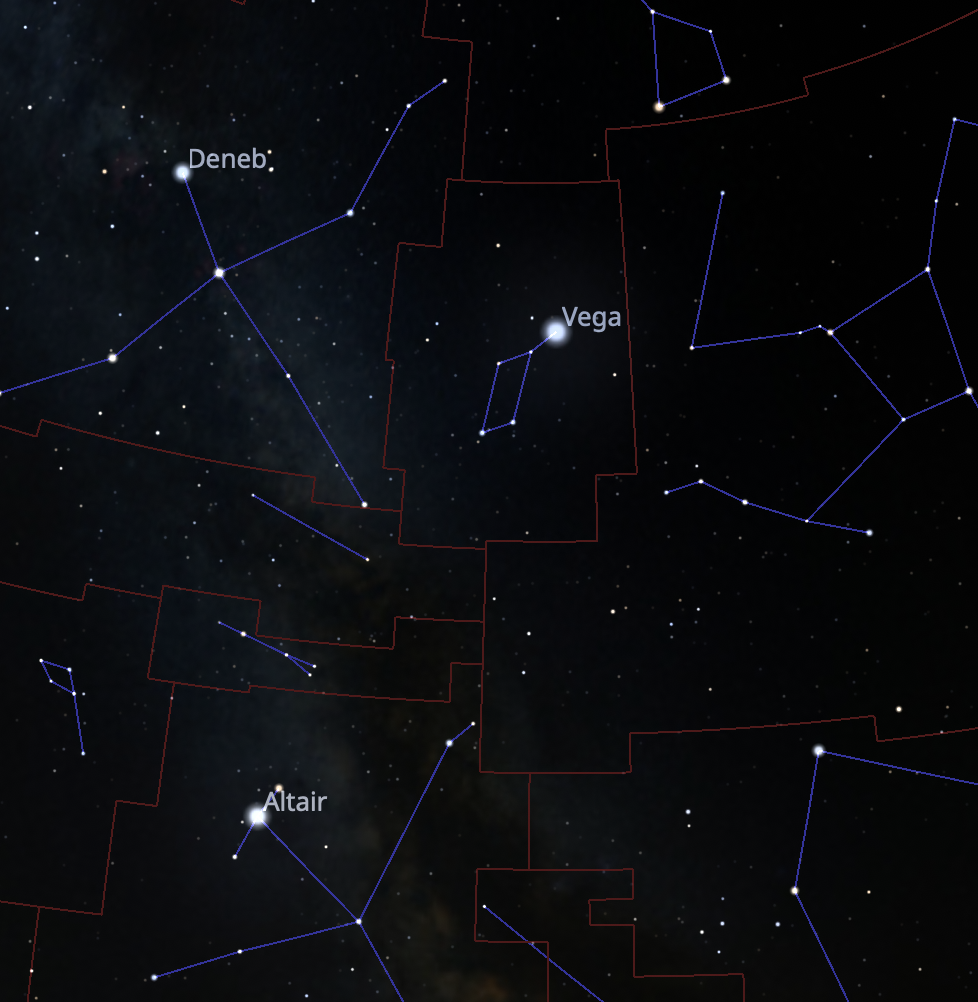
\includegraphics[width=12cm]{Resources/img/image.png}
    \caption{Fotografía realizada en Stellarium}{Detalles: Tiempo de exposición $t = 45 \ \text{yrs}$}\\{JD1293719823.2}.
    \label{fig:constelaciones}
\end{figure*}

Do et irure do pariatur elit amet. \ref{fig:constelaciones} Et aute proident duis in elit eiusmod aliquip ipsum ullamco do voluptate.


\subsection{Pregunta 3} \label{subsec:pregunta3}

\noindent \textbf{Pregunta} 

Duis pariatur velit amet enim amet ea irure ullamco laborum nulla enim voluptate.

\begin{enumerate}
    \item[a)] Duis pariatur velit amet enim amet ea irure ullamco laborum nulla enim voluptate
    \item[b)] Duis pariatur velit amet enim amet ea irure ullamco laborum nulla enim voluptate
    \item[c)] Duis pariatur velit amet enim amet ea irure ullamco laborum nulla enim voluptate
\end{enumerate}

\noindent \textbf{Desarrollo} 

Duis pariatur velit amet enim amet ea irure ullamco laborum nulla enim voluptate.


\begin{figure*}[ht!]
    \gridline{\fig{Resources/tikz/output/all.pdf}{0.4\textwidth}{Solución a)}
              \fig{Resources/tikz/output/lat.pdf}{0.4\textwidth}{Solución b)}}
    \gridline{\fig{Resources/tikz/output/alt.pdf}{0.4\textwidth}{Solución c)}
              \fig{Resources/tikz/output/all.pdf}{0.4\textwidth}{Vista General}}
    \centering
    \caption{Eiusmod proident est labore occaecat cupidatat reprehenderit ut amet proident do consequat sunt. \ref{subsec:pregunta3}}
    {Esse in fugiat velit voluptate duis nulla.}
    \label{fig:pregunta3desarrollo}
\end{figure*}


\subsection{Pregunta 4} \label{subsec:pregunta4}
\noindent \textbf{Pregunta} 

``Veniam dolore aliqua ea mollit sunt aute esse."

\noindent \textbf{Respuesta}

Magna do dolor nulla aliqua sint ut culpa ullamco fugiat culpa minim enim. Non reprehenderit fugiat aliqua fugiat enim elit officia id sint. Duis amet ipsum dolor deserunt voluptate dolore incididunt laboris enim id elit aliqua id. Fugiat officia amet dolore proident proident.

Quis officia sit aliqua sint. Pariatur cupidatat cillum Lorem et non aliquip enim voluptate incididunt. Est consequat dolore minim laboris ut mollit laboris. Occaecat occaecat exercitation dolore laboris ad exercitation velit enim ut elit duis anim sint. Et dolore pariatur nostrud cillum sit ex minim.


\noindent \textbf{Pregunta}
``Quis sit labore elit ipsum excepteur.''

\noindent \textbf{Respuesta}
Eu ex ad deserunt laborum aute laborum culpa enim ipsum eu nisi. Ex enim id consequat in ex in velit pariatur tempor. Ipsum aute aliqua enim ut est dolore aliquip ipsum sint proident ut ad. Aliquip ex minim ex pariatur veniam tempor pariatur ea reprehenderit Lorem nisi ex enim.

Quis eiusmod nisi dolore proident labore sit ipsum minim ad veniam magna ea nisi. Officia et commodo ea eu in. Occaecat ullamco eiusmod sint occaecat. Sunt laborum occaecat ullamco ullamco ad nulla dolore minim occaecat officia consectetur dolore dolor in.

Et occaecat officia anim fugiat aliqua commodo et anim minim nulla tempor ipsum anim laborum. Esse proident reprehenderit ad proident consectetur officia labore nulla deserunt non ex. Occaecat incididunt do ad id sit aliqua. Tempor esse esse irure anim cillum sunt non ipsum elit mollit veniam. Elit quis ex Lorem cupidatat eu occaecat enim sint. Non ut aliqua elit enim labore ut nostrud culpa elit labore. Do laborum consequat occaecat est minim labore proident consectetur mollit aute ut.

Nostrud eu fugiat adipisicing incididunt. Eiusmod commodo pariatur esse sunt occaecat ullamco excepteur sint irure. Pariatur esse ad consequat ut aliqua in ut culpa consequat. Sint Lorem occaecat exercitation velit ad irure duis aute deserunt. Ad ipsum id cillum eu excepteur do laboris.

% Planck's Law Derivation (Equations Only with \[ \])

\[
E_n = n h \nu \quad \text{with} \quad n = 0, 1, 2, \dots
\]

\[
\langle E \rangle = \frac{\sum_{n=0}^{\infty} E_n e^{-E_n / k_B T}}{\sum_{n=0}^{\infty} e^{-E_n / k_B T}}
\]

\[
\langle E \rangle = \frac{\sum_{n=0}^{\infty} n h \nu e^{-n h \nu / k_B T}}{\sum_{n=0}^{\infty} e^{-n h \nu / k_B T}}
\]

\[
\langle E \rangle = \frac{h \nu}{e^{h \nu / k_B T} - 1}
\]

\[
u(\nu, T) = \frac{8 \pi \nu^2}{c^3} \langle E \rangle
\]

\[
u(\nu, T) = \frac{8 \pi h \nu^3}{c^3} \cdot \frac{1}{e^{h \nu / k_B T} - 1}
\]

\[
u(\lambda, T) = \frac{8 \pi h c}{\lambda^5} \cdot \frac{1}{e^{h c / \lambda k_B T} - 1}
\]


% \section{A short history of AASTeX} 

\latex\ \footnote{\url{http://www.latex-project.org/}} is a document markup
language that is particularly well suited for the publication of
mathematical and scientific articles \citep{lamport94}. \latex\ was written
in 1985 by Leslie Lamport who based it on the \TeX\ typesetting language
which itself was created by Donald E. Knuth in 1978.  In 1988 a suite of
\latex\ macros were developed to investigate electronic submission and
publication of AAS Journal articles \citep{1989BAAS...21..780H}.  Shortly
afterwards, Chris Biemesdefer merged these macros and more into a \latex\
2.08 style file called \aastex.  These early \aastex\ versions introduced
many common commands and practices that authors take for granted today.
Substantial revisions
were made by Lee Brotzman and Pierre Landau when the package was updated to
v4.0.  AASTeX v5.0, written in 1995 by Arthur Ogawa, upgraded to \latex\ 2e
which uses the document class in lieu of a style file.  Other improvements
to version 5 included hypertext support, landscape deluxetables and
improved figure support to facilitate electronic submission.  
\aastex\ v5.2 was released in 2005 and introduced additional graphics
support plus new mark up to identifier astronomical objects, datasets and
facilities.

In 1996 Maxim Markevitch modified the AAS preprint style file, aaspp4.sty,
to closely emulate the very tight, two column style of a typeset
Astrophysical Journal article.  The result was emulateapj.sty. A year
later Alexey Vikhlinin took over development and maintenance\footnote{\url{https://hea-www.harvard.edu/~alexey/emulateapj/}}. In 2001 he
converted emulateapj into a class file in \latex\ 2e and in 2003 Vikhlinin
completely rewrote emulateapj based on the APS Journal's REVTEX class.

During this time emulateapj gained growing acceptance in the astronomical
community as it filled an author need to obtain an approximate number of
manuscript pages prior to submission for cost and length estimates. The
tighter typeset also had the added advantage of saving paper when printing 
hard copies.

%% The "ht!" tells LaTeX to put the figure "here" first, at the "top" next
%% and to override the normal way of calculating a float position.
%% The asterisk after "figure" tells the compiler to span multiple columns
%% if a two column style is selected.
\begin{figure*}[ht!]
\plotone{Resources/img/AuthorChargeInfographic.png}
\caption{The AAS journals are operated as a nonprofit venture, and author charges fairly recapture costs for the services provided in the publishing process. The chart above breaks down the services that author charges go toward. The AAS Journals' Business Model is outlined in a \href{https://aas.org/posts/news/2023/08/aas-open-access-publishing-model-open-transparent-and-fair}{2023 post}.
\label{fig:general}}
\end{figure*}

Even though author publication charges where no longer based on print pages
\footnote{see Section \ref{sec:pubcharge} in the Appendix for more details
about how current article costs are calculated. Figure \ref{fig:general} shows
how author publication charges are currently spent.} the emulateapj class file
proved to be extremely popular with AAS Journal authors.  An 
analysis of submitted \latex\ manuscripts in 2015 revealed that $\sim$30\%
either called emulateapj or had a commented emulateapj classfile call
indicating it was used at some stage of the manuscript construction.
Clearly authors wanted to have access to a tightly typeset version of the
article when editing with co-authors and for preprint submissions.

When planning the next \aastex\ release the popularity of emulateapj played
an important roll in the decision to drop the old base code and adopt and
modify emulateapj for \aastex\ v6.+.  Those changes brought \aastex\
inline with what the majority of authors are already using while still
delivering new and improved features.  \aastex\ v6.0 through v6.31 were
developted by Amy Hendrickson\footnote{\url{https://www.texnology.com/about.htm}}.
The release dates for the \aastex 6 versions were January 2016 (v6.0),
October 2016 (v6.1), January 2018 (v6.2), June 2019 (v6.3), and March 2020
(v6.3.1), respectively.

\aastex\'s reliance on REVTeX, specifically v4-1, proved to be problematic when it was superseded in in January 2019. Rather than continue with REVTeX v4-2 as the base package of \aastex, Aptara\footnote{\url{https://www.aptaracorp.com}} was hire to rewrite \aastex from scratch while keeping the core functionality in early 2024. This new version, v7.0, was released in January 2025. Users of v6.3.1 will have little difficulty migrating to this new version with the core difference being that an email address is required for each author in v7.

The rest of this article provides information and examples on how to create
your own AAS Journal manuscript with v7.  Special emphasis is placed on
how to use the full potential of \aastex. Note that some of the examples are commented out in this latex manuscript. The next section describes
the different manuscript styles available.
Section \ref{sec:floats} describes table and figure placement. 
Specific examples of different table are provided,  Section
\ref{subsec:tables}.
Section \ref{sec:highlight}
discuss how to properly highlight text added during revisions.  
The last section,
\ref{sec:cite}, shows how to recognize software and external data as first
class references in the manuscript bibliography.  An appendix is included
for additional information readers might find useful.
More documentation is embedded in the comments of this \latex\ file and in the online documentation at
\url{http://journals.aas.org/authors/aastex.html}.
% \section{Manuscript styles} \label{sec:style}

The default style in \aastex\ v7 is a tight single column style, e.g. 10
point font, single spaced.  The single column style is very useful for
article with wide equations. It is also the easiest to style to work with
since figures and tables, see Section \ref{sec:floats}, will span the
entire page, reducing the need for address float sizing.

To invoke a two column style similar to the what is produced in
the published PDF copy use \\

\noindent {\tt\string\documentclass[twocolumn]\{aastex7\}}. \\

\noindent Note that in the two column style figures and tables will only
span one column unless specifically ordered across both with the ``*'' flag,
e.g. \\

\noindent{\tt\string\begin\{figure*\}} ... {\tt\string\end\{figure*\}}, \\
\noindent{\tt\string\begin\{table*\}} ... {\tt\string\end\{table*\}}, and \\
\noindent{\tt\string\begin\{deluxetable*\}} ... {\tt\string\end\{deluxetable*\}}. \\

\noindent This option is ignored in the {\tt\string onecolumn} style.

All authors should have the {\tt\string linenumbers} style include so that
the compiled PDF has each row numbered in the left margin. Line numbering
is mandatory as it helps reviewers quickly identify locations in the text.

The {\tt\string anonymous} option will prevent the author and affiliations
from being shown in the compiled pdf copy. This option allows the author 
to keep this critical information in the latex file but prevent the reviewer
from seeing it during peer review if dual anonymous review (DAR) is requested. 
Likewise, acknowledgments and author contributions can also be hidden if placed in the {\tt\string\begin\{acknowledgments\}} ... {\tt\string\end\{acknowledgments\}} and {\tt\string\begin\{contribution\}} ... {\tt\string\end\{contribution\}} environments. The use of this option is highly recommended for PSJ submissions. Advice for anonymizing your manuscript for DAR is provided at 
\url{https://journals.aas.org/manuscript-preparation/#dar}.

Another reason to use the {\tt\string\begin\{acknowledgments\}} ... {\tt\string\end\{acknowledgments\}} and {\tt\string\begin\{contribution\}} ... {\tt\string\end\{contribution\}} environments is that the word counter in our peer review system will \textbf{not} count the contents of these environments. If authors put aknowledgments and contribution text in other locations, these words will be counter and authors may be overcharged on their author publication charges.

Multiple style options are allowed, e.g. \\

\noindent {\tt\string\documentclass[linenumbers,trackchanges,anonymous]\{aastex7\}}. \\

% \section{Floats} \label{sec:floats}

Floats are non-text items that generally can not be split over a page.  They also have captions and can be numbered for reference.  Primarily these are figures and tables but authors can define their own. \latex\ tries to place a float where indicated in the manuscript but will move it later if there is not enough room at that location, hence the term ``float''.

Authors are encouraged to embed their tables and figures within the text as they are mentioned.  Editors and the vast majority of referees find it much easier to read a manuscript with embedded figures and tables.

Depending on the number of floats and the particular amount of text and equations present in a manuscript the ultimate location of any specific float can be hard to predict prior to compilation. It is recommended that authors \textbf{not} spend significant time trying to get float placement perfect for peer review.  The AAS Journal's publisher has sophisticated typesetting software that will produce the optimal layout during production.

Note that authors of Research Notes are only allowed one float, either one table or one figure.

For authors that do want to take the time to optimize the locations of their floats there are some techniques that can be used.  The simplest solution is to placing a float earlier in the text to get the position right but this option will break down if the manuscript is altered.  A better method is to force \latex\ to place a float in a general area with the use of the optional {\tt\string [placement specifier]} parameter for figures and tables. This parameter goes after {\tt\string \begin\{figure\}}, {\tt\string \begin\{table\}}, and {\tt\string \begin\{deluxetable\}}.  The main arguments the specifier takes are ``h'', ``t'', ``b'', and ``!''.  These tell \latex\ to place the float \underline{h}ere (or as close as possible to this location as possible), at the \underline{t}op of the page, and at the \underline{b}ottom of the page.  The last argument, ``!'', tells \latex\ to override its internal method of calculating the float position.  A sequence of rules can be created by using multiple arguments.  For example, {\tt\string \begin\{figure\}[htb!]} tells \latex\ to try the current location first, then the top of the page and finally the bottom of the page without regard to what it thinks the proper position should be.  Many of the tables and figures in this article use a placement specifier to set their positions.

Note that the \latex\ {\tt\string tabular} environment is not a float.  Only when a {\tt\string tabular} is surrounded by {\tt\string\begin\{table\}} ...  {\tt\string\end\{table\}} is it a true float and the rules and suggestions above apply.

In AASTeX all deluxetables are float tables and thus if they are longer than a page will spill off the bottom. Long deluxetables should begin with the {\tt\string\startlongtable} command. This initiates a longtable environment.  Authors might have to use {\tt\string\clearpage} to isolate a long table or optimally place it within the surrounding text.

\subsection{Tables} \label{subsec:tables}

Tables can be constructed with \latex's standard table environment or the \aastex's deluxetable environment. The deluxetable construct handles long tables better but has a larger overhead due to the greater amount of defined mark up used set up and manipulate the table structure.  The choice of which to use is up to the author.  Examples of both environments are used in this manuscript. 

Tables longer than 200 data lines and complex tables should only have a short example table with the full data set available in the machine readable format.  The machine readable table will be available in the HTML version of the article with just a short example in the PDF. Authors are required to indicate in the table comments that the data in machine readable format in the full article.  Authors are encouraged to create their own machine readable tables using the online tool at \url{http://authortools.aas.org/MRT/upload.html}.

\aastex\ v6 introduced five new table features that were designed to make
table construction easier and the resulting display better for AAS Journal
authors. The items are:

\begin{enumerate}
\item Declaring math mode in specific columns,
\item Column decimal alignment, 
\item Automatic column header numbering,
\item Hiding columns, and
\item Splitting wide tables into two or three parts.
\end{enumerate}

Full details on how to create each of these special table types are given in the guidelines at \url{http://journals.aas.org/authors/aastex.html}.

\subsubsection{Extremely wide tables}

Since the AAS Journals are now all electronic with no print version there is no reason why tables can not be as wide as authors need them to be. For wide tables, the full table will almost always be available in machine readalbe format with just an example in the article but how is an example created for a wide table?

There are two ways to create examples for wide tabular data sets. The first is to to break a table into two or three components so that it flows down a page by invoking a new table type, splittabular or splitdeluxetable. Within these tables a new ``B'' column separator is introduced.  Much like the vertical bar option, ``$\vert$'', that produces a vertical table lines the new ``B'' separator indicates where to \underline{B}reak a table.  Up to two ``B''s may be included.

Table 1 shows how to split a wide deluxetable into three parts with
the {\tt\string\splitdeluxetable} command.  The {\tt\string\colnumbers}
option is on to show how the automatic column numbering carries through the
second table component.

\begin{splitdeluxetable*}{lccccBcccccBcccc}
\tabletypesize{\scriptsize}
\tablewidth{0pt} 
\tablecaption{Measurements of Emission Lines: two breaks \label{tab:deluxesplit}}
\tablehead{
\colhead{Model} & \colhead{Component}& \colhead{Shift} & \colhead{FWHM} &
\multicolumn{10}{c}{Flux} \\
\colhead{} & \colhead{} & \colhead{($\rm
km~s^{-1}$)}& \colhead{($\rm km~s^{-1}$)} & \multicolumn{10}{c}{($\rm
10^{-17}~erg~s^{-1}~cm^{-2}$)} \\
\cline{5-14}
\colhead{} & \colhead{} &
\colhead{} & \colhead{} & \colhead{Ly$\alpha$} & \colhead{N\,{\footnotesize
V}} & \colhead{Si\,{\footnotesize IV}} & \colhead{C\,{\footnotesize IV}} &
\colhead{Mg\,{\footnotesize II}} & \colhead{H$\gamma$} & \colhead{H$\beta$}
& \colhead{H$\alpha$} & \colhead{He\,{\footnotesize I}} &
\colhead{Pa$\gamma$}
} 
\colnumbers
\startdata 
{       }& BELs& -97.13 &    9117$\pm      38$&    1033$\pm      33$&$< 35$&$<     166$&     637$\pm      31$&    1951$\pm      26$&     991$\pm 30$&    3502$\pm      42$&   20285$\pm      80$&    2025$\pm     116$& 1289$\pm     107$\\ 
{Model 1}& IELs& -4049.123 & 1974$\pm      22$&    2495$\pm      30$&$<     42$&$<     109$&     995$\pm 186$&      83$\pm      30$&      75$\pm      23$&     130$\pm      25$& 357$\pm      94$&     194$\pm      64$& 36$\pm      23$\\
{       }& NELs& \nodata &     641$\pm       4$&     449$\pm 23$&$<      6$&$<       9$&       --            &     275$\pm      18$& 150$\pm      11$&     313$\pm      12$&     958$\pm      43$&     318$\pm 34$& 151$\pm       17$\\
\hline
{       }& BELs& -85 &    8991$\pm      41$& 988$\pm      29$&$<     24$&$<     173$&     623$\pm      28$&    1945$\pm 29$&     989$\pm      27$&    3498$\pm      37$&   20288$\pm      73$& 2047$\pm     143$& 1376$\pm     167$\\
{Model 2}& IELs& -51000 &    2025$\pm      26$& 2494$\pm      32$&$<     37$&$<     124$&    1005$\pm     190$&      72$\pm 28$&      72$\pm      21$&     113$\pm      18$&     271$\pm      85$& 205$\pm      72$& 34$\pm      21$\\
{       }& NELs& 52 &     637$\pm      10$&     477$\pm 17$&$<      4$&$<       8$&       --            &     278$\pm      17$& 153$\pm      10$&     317$\pm      15$&     969$\pm      40$&     325$\pm 37$&
     147$\pm       22$\\
\enddata
\tablecomments{This is an example of how to split a deluxetable. You can
split any table with this command into two or three parts.  The location of
the split is given by the author based on the placement of the ``B''
indicators in the column identifier preamble.  For more information please
look at the new \aastex\ instructions.}
\end{splitdeluxetable*}

The second way is to create a "descriptive" table instead. This type of table only provides information about the columns rather than the data itself. Table 2 shows an example of this type of table using the same columns as in Table 1. Since these types of tables always have a machine readable component, this table uses the {\tt\string \digitalasset}\ command to highlight this fact.

\begin{deluxetable*}{rlll}
\digitalasset
\tablewidth{0pt}
\tablecaption{Descriptive version of the "Measurements of Emission Lines" table \label{tab:description}}
\tablehead{
\colhead{Number} & \colhead{Units} & \colhead{Label} & \colhead{Explanation}
}
\startdata
1 & --- & Model & Model identifier \\
2 & --- & Component & Component identifier \\
3 & $\rm km~s^{-1}$ & Shift & Line shift \\
4 & $\rm km~s^{-1}$ & FWHM & Line Full-Width at Half-Maximum \\
5 & $\rm 10^{-17}~erg~s^{-1}~cm^{-2}$ & Ly$\alpha$ & Ly$\alpha$ line flux \\
6 & $\rm 10^{-17}~erg~s^{-1}~cm^{-2}$ & N\,{\footnotesize V} & N\,{\footnotesize V} line flux \\
7 & $\rm 10^{-17}~erg~s^{-1}~cm^{-2}$ & Si\,{\footnotesize IV} & Si\,{\footnotesize IV} line flux \\
8 & $\rm 10^{-17}~erg~s^{-1}~cm^{-2}$ & C\,{\footnotesize IV} & C\,{\footnotesize IV} line flux \\
9 & $\rm 10^{-17}~erg~s^{-1}~cm^{-2}$ & Mg\,{\footnotesize II} & Mg\,{\footnotesize II} line flux \\
10 & $\rm 10^{-17}~erg~s^{-1}~cm^{-2}$ & H$\gamma$ & H$\gamma$ line flux \\
11 & $\rm 10^{-17}~erg~s^{-1}~cm^{-2}$ & H$\beta$ & H$\beta$ line flux \\
12 & $\rm 10^{-17}~erg~s^{-1}~cm^{-2}$ & H$\alpha$ & H$\alpha$ line flux \\
13 & $\rm 10^{-17}~erg~s^{-1}~cm^{-2}$ & He\,{\footnotesize I} & He\,{\footnotesize I} line flux \\
14 & $\rm 10^{-17}~erg~s^{-1}~cm^{-2}$ & Pa$\gamma$ & Pa$\gamma$ line flux \\
\enddata
\tablecomments{Table 2 is published in its entirety in the electronic 
edition of the {\it Astrophysical Journal}.  A portion is shown here 
for guidance regarding its form and content. The {\tt\string \digitalasset}\ command highlights the Table title to visually indicate to the reader that there is data associated with this table.}
\end{deluxetable*}

\subsection{Figures\label{subsec:figures}}

Authors can include a wide number of different graphics with their articles.
These range from general figures all authors are familiar with
to new enhanced graphics that can only be fully experienced in HTML.  The
later include figure sets, animations and interactive figures.  All
enhanced graphics require a static two dimensional representation in the
manuscript to serve as the example for the reader. All figures should
include detailed and descriptive captions.  These captions are absolutely
critical for readers for whom the enhanced figure is inaccessible either
due to a disability or offline access.  This portion of the article
provides examples for setting up all these types in with the latest version
of \aastex.

\subsection{General figures\label{subsec:general}}

\aastex\ has a {\tt\string\plotone} command to display a figure consisting
of one figure file.  Figure \ref{fig:general} is an example which shows
how AAS Publishing spends author publication charges. For a general figure
consisting of two figure files the {\tt\string\plottwo} command can be
used to position the two image files side by side.

Both {\tt\string\plotone} and {\tt\string\plottwo} take a
{\tt\string\caption} and an optional {\tt\string\figurenum} command to
specify the figure number\footnote{It is better to not use
{\tt\string\figurenum} and let \latex\ auto-increment all the figures. If you
do use this command you need to mark all of them accordingly.}.  Each is
based on the {\tt\string graphicx} package command,
{\tt\string\includegraphics}.  Authors are welcome to use
{\tt\string\includegraphics} along with its optional arguments that control
the height, width, scale, and position angle of a file within the figure.
More information on the full usage of {\tt\string\includegraphics} can be
found at \break
\url{https://en.wikibooks.org/wiki/LaTeX/Importing\_Graphics\#Including\_graphics}.

\subsection{Enhanced graphics}

Enhanced graphics have an example figure to serve as an example for the
reader and the full graphical item available in the published HTML article.
This includes Figure sets, animations, and interactive figures. The 
Astronomy Image Explorer (\url{http://www.astroexplorer.org/}) provides 
access to all the figures published in the AAS Journals since they offered
an electronic version which was in the mid 1990s. You can filter image
searches by specific terms, year, journal, or type. The type filter is 
particularly useful for finding all published enhanced graphics. As of
August 2024 there are over 5600 videos, 2200 figure sets, and 200 interactive
figures. The next sections describe how to include these types of graphics
in your own manuscripts.

% \section{Revision tracking and color highlighting} \label{sec:highlight}

The {\tt\string\added\{<text>\}} command should be used to highlight new text in bold for revised manuscripts. To activate this command, the {\tt\string trackchanges} option must be used in the {\tt\string\documentclass} call.  When compiled this will produce the marked text in bold font. Take out the {\tt\string trackchanges} option if you want the bold to disappear.

\added{This text was specifically added to feature this reborn functionality. Notice how the bold goes away when you remove the 'trackfeatures' option.}

% \section{Software and third party data repository citations} \label{sec:cite}

The AAS Journals would like to encourage authors to change software and
third party data repository references from the current standard of a
footnote to a first class citation in the bibliography.  As a bibliographic
citation these important references will be more easily captured and credit
will be given to the appropriate people.

The first step to making this happen is to have the data or software in
a long term repository that has made these items available via a persistent
identifier like a Digital Object Identifier (DOI).  A list of repositories
that satisfy this criteria plus each one's pros and cons are given at \break
\url{https://github.com/AASJournals/Tutorials/tree/master/Repositories}.

In the bibliography the format for data or code follows this format: \\

\noindent author year, title, version, publisher, prefix:identifier\\

\citet{2015ApJ...805...23C} provides a example of how the citation in the
article references the external code at
\doi{10.5281/zenodo.15991}.  Unfortunately, bibtex does
not have specific bibtex entries for these types of references so the
``@misc'' type should be used.  The Repository tutorial explains how to
code the ``@misc'' type correctly.  The most recent .bst file, aasjournalv7.bst, will output bibtex ``@misc'' type properly.

Authors can also use the website \url{https://www.doi2bib.org/} to create a BIBTeX entry for any DOI. Please check the output from this site carefully as its output is only as good as the DOI metadata. Some DOI creators do not provide enough metadata to construct an adequate citation.



%% [UC-TeX] ====================================== ACKNOWLEDGMENT & CONTRIBUTIONS =========================================
%% [AASTeX] Please use the acknowledgment and contribution environments. This will 
%% [AASTeX] be anonomyized when the "anonymous" style option is used. 

%% [UC-TeX][INPUT] 

\begin{acknowledgments}[Comentarios]

\end{acknowledgments}
% \begin{contribution}
    %%This section gives authors the space to recognize author contributions. The text inside this environment is NOT counted towards the total word quanta. At a minimum, manuscripts are expected to include this text:
    
    All authors contributed equally to the Terra Mater collaboration.
    
    %% But authors are expected to provide more specific details, e.g. 
    %%
    %%SC was responsible for writing and submitting the manuscript.
    %%WWM came up with the initial research concept and edited the manuscript.
    %%OTS obtained the funding and edited the manuscript.
    %%EBF provided the formal analysis and validation. He also edited the manuscript.
    %%GEH Supervised the undergraduates, wrote the software and administers the project github and Zenodo repositories.
    %%
    %% Authors can use the Contributor Role Taxonomy (CRediT) at
    %% https://credit.niso.org
    %% for ideas on how write a good statement tailored to their needs.
    
    \end{contribution}

%% [UC-TeX] ============================================== FACILITIES ====================================================
%% [AASTeX] To help institutions obtain information on the effectiveness of their 
%% [AASTeX] telescopes the AAS Journals has created a group of keywords for telescope 
%% [AASTeX] facilities.
%% [AASTeX] 
%% [AASTeX] Following the acknowledgments section, use the following syntax and the
%% [AASTeX] \facility{} or \facilities{} macros to list the keywords of facilities used 
%% [AASTeX] in the research for the paper.  Each keyword is check against the master 
%% [AASTeX] list during copy editing.  Individual instruments can be provided in 
%% [AASTeX] parentheses, after the keyword, but they are not verified.

%% [UC-TeX][INPUT] 
%% [UC-TeX] You may add more, {Fac1, Fac2, Fac3}...
\facilities{OUC (Santa Martina)}

%% [UC-TeX] ================================================ SOFTWARE ====================================================
%% [AASTeX] Similar to \facility{}, there is the optional \software command to allow 
%% [AASTeX] authors a place to specify which programs were used during the creation of 
%% [AASTeX] the manuscript. Authors should list each code and include either a
%% [AASTeX] citation or url to the code inside ()s when available.

%% [UC-TeX][INPUT] 
%% [UC-TeX] You may add more, {Soft1, Soft2, Soft3}...
\software{Siril \citep{Richard2024},
          Stellarium \citep{Zotti_Wolf_2022},
          \texttt{tikz3dtools} \citep{tikz3dtools},
          }

%% [UC-TeX] ============================================== APENDIX ======================================================
%% [AASTeX] Appendix material should be preceded with a single \appendix command.
%% [AASTeX] There should be a \section command for each appendix. Mark appendix
%% [AASTeX] subsections with the same markup you use in the main body of the paper.
%% [AASTeX] 
%% [AASTeX] Each Appendix (indicated with \section) will be lettered A, B, C, etc.
%% [AASTeX] The equation counter will reset when it encounters the \appendix
%% [AASTeX] command and will number appendix equations (A1), (A2), etc. The
%% [AASTeX] Figure and Table counter will not reset.

%% [UC-TeX][INPUT] 
%% [UC-TeX] Uncomment to display appendix
% \appendix

% \section{Appendix information}

Appendices can be broken into separate sections just like in the main text.
The only difference is that each appendix section is indexed by a letter
(A, B, C, etc.) instead of a number.  Likewise numbered equations have
the section letter appended.  Here is an equation as an example.
\begin{equation}
I = \frac{1}{1 + d_{1}^{P (1 + d_{2} )}}
\end{equation}
Appendix tables and figures should not be numbered like equations. Instead
they should continue the sequence from the main article body.
% \section{Author publication charges} \label{sec:pubcharge}

In April 2011 the traditional way of calculating author charges based on 
the number of printed pages was changed.  The reason for the change
was due to a recognition of the growing number of article items that could not 
be represented in print. Now author charges are determined by a number of
digital ``quanta''.  A single quantum is defined as 350 words, one figure, one table,
and one digital asset.  For the latter this includes machine readable
tables, data behind a figure, figure sets, animations, and interactive figures.  The current cost
for the different quanta types is available at 
\url{https://journals.aas.org/article-charges-and-copyright/#author_publication_charges}. 
Authors may use the ApJL length calculator to get a {\tt rough} estimate of 
the number of word and float quanta in their manuscript. The calculator 
is located at \url{https://authortools.aas.org/ApJL/betacountwords.html}.
% \section{Rotating tables} \label{sec:rotate}

To place a single page table in a landscape mode start the table portion with {\tt\string\begin\{rotatetable\}} and end with {\tt\string\end\{rotatetable\}}.

Tables that exceed a print page take a slightly different environment since both rotation and long table printing are required. In these cases start with {\tt\string\begin\{longrotatetable\}} and end with {\tt\string\end\{longrotatetable\}}. The {\tt\string\movetabledown} command can be used to help center extremely wide, landscape tables. The command {\tt\string\movetabledown=1in} will move any rotated table down 1 inch. 

A handy "cheat sheet" that provides the necessary \latex\ to produce 17
different types of tables is available at \url{http://journals.aas.org/authors/aastex/aasguide.html#table_cheat_sheet}.

% \section{Using Chinese, Japanese, and Korean characters}

Authors have the option to include names in Chinese, Japanese, or Korean (CJK)
characters in addition to the English name. The names will be displayed
in parentheses after the English name. The way to do this in AASTeX is to
use the CJK package available at \url{https://ctan.org/pkg/cjk?lang=en}.
Further details on how to implement this and solutions for common problems,
please go to \url{https://journals.aas.org/nonroman/}.


%% [UC-TeX] ============================================== BIBLIOGRAPHY ==================================================
%% [AASTeX] [For this sample we use BibTeX plus aasjournalv7.bst to generate the
%% [AASTeX] the bibliography. The sample7.bib file was populated from ADS. To
%% [AASTeX] get the citations to show in the compiled file do the following:
%% [AASTeX] 
%% [AASTeX] pdflatex sample7.tex
%% [AASTeX] bibtext sample7
%% [AASTeX] pdflatex sample7.tex
%% [AASTeX] pdflatex sample7.tex

%% [UC-TeX] Change Informe if you have a different name for your bib file
%% [UC-TeX][INPUT] 
\bibliography{Informe}{}
\bibliographystyle{Config/NoMod/aasjournalv7.bst}

%% [AASTeX] This command is needed to show the entire author+affiliation list when
%% [AASTeX] the collaboration and author truncation commands are used.  It has to
%% [AASTeX] go at the end of the manuscript.

%% [UC-TeX] Uncomment to display all authors
%\allauthors

%% [AASTeX] Include this line if you are using the \added, \replaced, \deleted
%% [AASTeX] commands to see a summary list of all changes at the end of the article.
%% [UC-TeX] Uncomment to display changes
%\listofchanges

\end{document}